
\section{Lexicographic Fréchet Distance with Degenerate Inputs}\label{lex_frechet_deg}

\subsection{Problem}

As \citeauthor{rotelex} describes in Section 7 of his paper \citetitle{rotelex} and as we hinted to in Section \ref{sec:lex_frechet_alg} of this paper, multiple critical events can occur for the same $\epsilon$.

Multiple critical events for the same $\epsilon$ turn out to be problematic, because as can be seen in Algorithm \ref{alg:lex_frechet_alg}, we assume the functions defined in Algorithm \ref{alg:lex_frechet_alg_req} return only one critical event, which will be traversed.

This section aims to answer the question of how to handle multiple critical events with the same critical $\epsilon$ by visualizing the problem and postulating an algorithm that decides which combination of critical events result in a lexicographic traversal. The basis of this section is Section 7 of \citeauthor{rotelex}'s paper \citetitle{rotelex}\cite{rotelex}.


\subsection{Examples}

In this subsection, four examples will be discussed, for which multiple critical events for the same critical $\epsilon$ require a decision on which of them should be traversed to result in a lexicographic traversal.


\subsubsection{Minimal Example: Traverse Both}
% https://abegehr.github.io/frechet/?p=(5_5)(8_5)(2_5)(5_5)&q=(5.5_3)(4.5_7)

\begin{figure}[H]
    \centering
    
    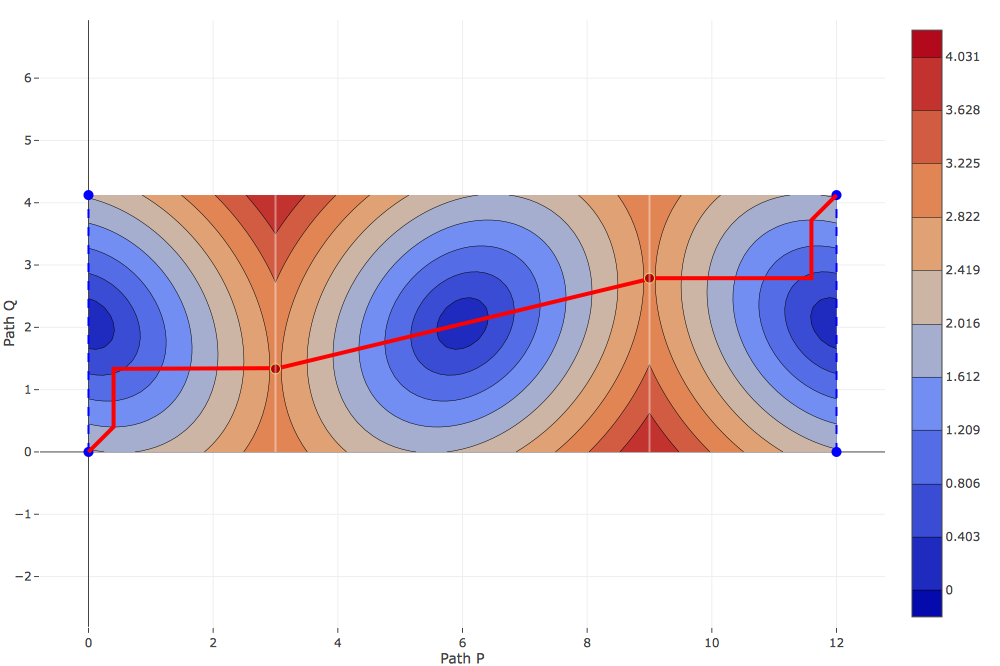
\includegraphics[width=0.8\textwidth]{ces_min_1_tra.png}
		
	\caption{Multiple critical events with same $\epsilon$. Traverse both.\protect\footnotemark}
    \label{fig:ces_min_1}
\end{figure}
\footnotetext{View the example here: \url{https://abegehr.github.io/frechet/?p=(5_5)(8_5)(2_5)(5_5)&q=(5.5_3)(4.5_7)}}

Figure \ref{fig:ces_min_1} shows a minimal example of multiple critical events for the same $\epsilon$. There are two classical critical events of type b with equal $\epsilon \approx 2.91$ at the two vertical cell-borders. It can be easily seen, that both need to be traversed.


\subsubsection{Minimal Example: Traverse Either One}
% https://abegehr.github.io/frechet/?p=(4_5)(8_5)(4_5)&q=(5_4)(5_7)(5_4)

\begin{figure}[H]
    \centering
    
    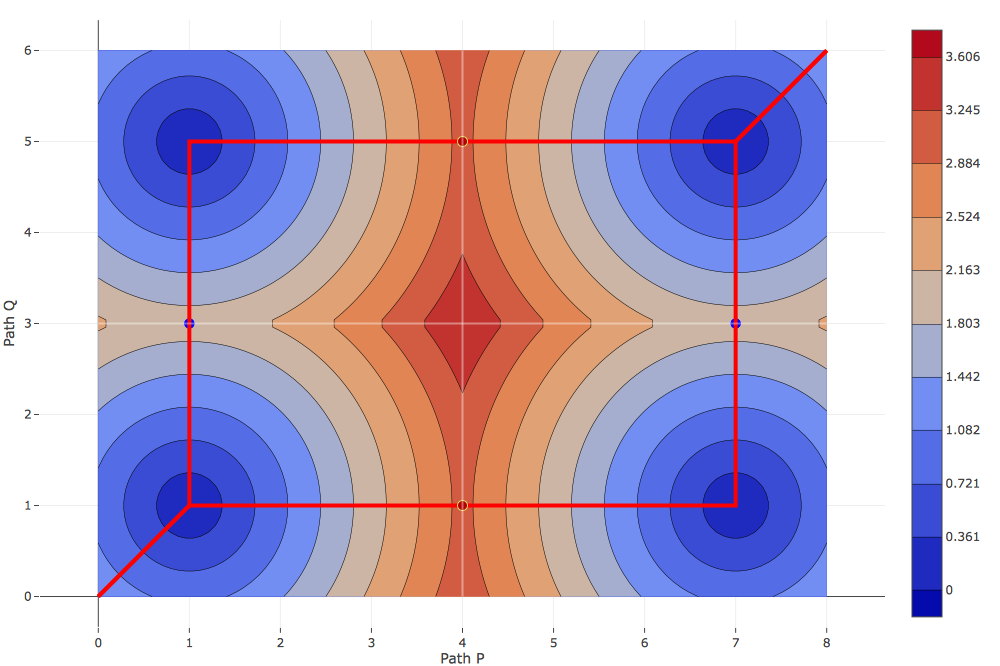
\includegraphics[width=0.8\textwidth]{ces_min_2_tra.png}
		
	\caption{Multiple critical events with same $\epsilon$. Traverse either one.\protect\footnotemark}
    \label{fig:ces_min_2}
\end{figure}
\footnotetext{View the example here: \url{https://abegehr.github.io/frechet/?p=(4_5)(8_5)(4_5)&q=(5_4)(5_7)(5_4)}}

Figure \ref{fig:ces_min_2} shows a minimal example of multiple critical events for the same $\epsilon$. There are four critical events to consider. Two classical critical events of type b with equal $\epsilon = 3$ at the two vertical cell-borders. And two classical critical events of type b with equal $\epsilon = 2$ at the two horizontal cell-borders. The decision problem shows that $\epsilon = 3$ is needed to traverse this $\delta$. It can be easily seen, that either one of the critical events at $\epsilon = 3$ need to be traversed.



\subsubsection{Minimal Example: Traverse One}
% https://abegehr.github.io/frechet/?p=(3_2)(3_8)(6_4)&q=(2_3)(8_3)(2_3)

\begin{figure}[H]
    \centering
    
    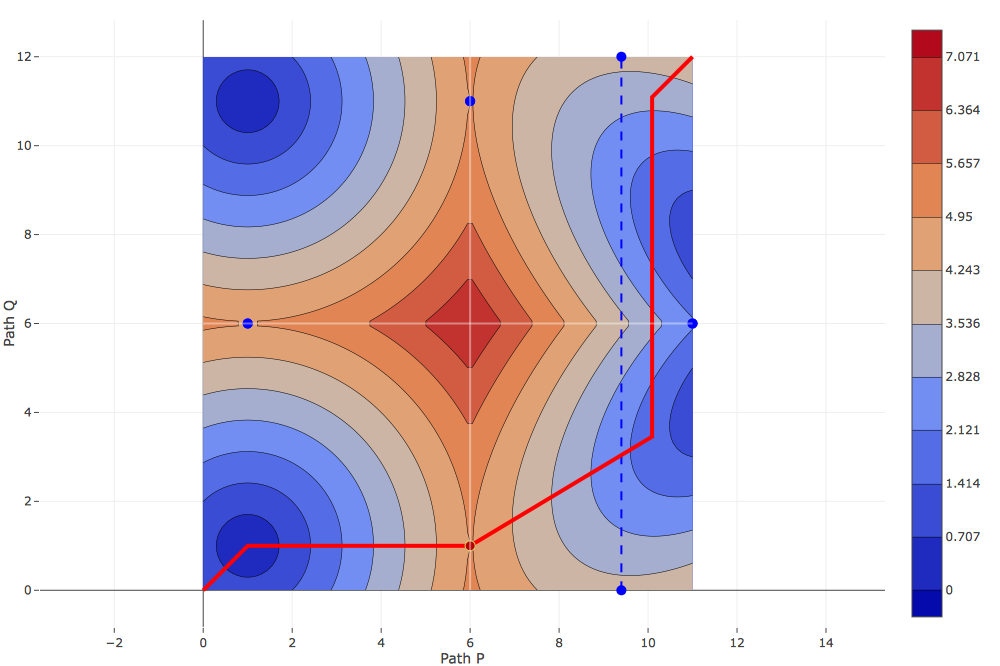
\includegraphics[width=0.8\textwidth]{ces_min_3_tra.png}
		
	\caption{Multiple critical events with same $\epsilon$. Traverse one.\protect\footnotemark}
    \label{fig:ces_min_3}
\end{figure}
\footnotetext{View the example here: \url{https://abegehr.github.io/frechet/?p=(3_2)(3_8)(6_4)&q=(2_3)(8_3)(2_3)}}

Figure \ref{fig:ces_min_3} shows a minimal example of multiple critical events for the same $\epsilon$. There are four critical events to consider. Two classical critical events of type b with equal $\epsilon = 3$ at the two vertical cell-borders. And two classical critical events of type b with equal $\epsilon = 2$ at the two horizontal cell-borders. The decision problem shows that $\epsilon = 3$ is needed to traverse this $\delta$. It can be easily seen, that either one of the critical events at $\epsilon = 3$ need to be traversed. !!!TODO!!!


\subsubsection{More Complex Example}

Figure \ref{fig:ces_com} shows a more complex example of multiple critical events for the same $\epsilon$. 



\subsection{Postulate Algorithm}
Postulate algorithm for choosing a critical event from several with equal epsilon: (visual examples!)

Algorithm:
\begin{enumerate}
	\item For every critical event compute reciprocal of derivates descents and store as critical event's steepness.
	\item From set of critical events, generate all possible sequences (ascending monotone).
	\item For all sequences sum steepness of their critical events and store as sequence rank.
	\item Starting with the smallest-rank sequence, decide if the sequence of critical events is traversable without passing critical events excluded in the sequence.
	\item If decision is negative, repeat 4.
	\item If decision is positive, repeat 4 for all sequences of equal rank.
	\item If multiple sequences of equal rank are found to be valid, traverse all, and decide by comparing.
	\item The steepness of the steepest decent.
	\item The steepness of critical event that is reached.
	\item And choose the path with the steepest summed recents of all paths.
	\item If multiple paths with same hight profile are found, return all. Otherwise return the lexicographic optimum.
	\item 
\end{enumerate}

\subsection{Traversing critical events}

Assume we are traversing a heat map generated by two curves. We arrive at a point where we have to decide which critical events need to be traversed for a lexicographic solution. The decision algorithm\cite{altgodau} can be applied for the $\epsilon$ of each possible critical event. We pick the smallest $\epsilon$ for which the decision algorithm returns a positive decision. We call it $\epsilon_0$. Now two options are feasible:

\begin{enumerate}[label=(\Alph*)]
	\item There is one critical event at height $\epsilon_0$. $|C_{\epsilon_0}| = 1$
	\item There are multiple critical events at height $\epsilon_0$. $|C_{\epsilon_0}| > 1$
\end{enumerate}

In case option A holds true, this critical event will need to be traversed. The traversal-problem is divided into two sub problems, which are both examined recursively and independently.

In case option B holds true, we need to decide which of the critical events $C_{\epsilon_0}$ need to be traversed and which are not needed for an optimal solution. We will consider all subsets $C'_{\epsilon_0}$ of $C_{\epsilon_0}$ with size $n>0$.

\subsubsection{Traversing multiple critical events with same $\epsilon$}

For each subset of critical events at $\epsilon_0$, $C'_{\epsilon_0} \subseteq C_{\epsilon_0}$ we compute if the critical events can be traversed monotonic. This can be done easily by applying the following procedure. For each critical event $C'_{\epsilon_0}(i)$, test if the start- and end-points of all other critical events in $C'_{\epsilon_0}$ are either lower-left of the starting point of $C'_{\epsilon_0}(i)$ or upper-right of the ending point of $C'_{\epsilon_0}(i)$.

See the a pseudocode for the function here. The function will return $True$ if the critical events $C'_{\epsilon_0}$ are traversable monotonically and $False$ if they are not.
\begin{algorithm}[H]
\caption{Critical Events $C'_{\epsilon_0}$ Monotonic Traversable}\label{euclid}
\begin{algorithmic}[1]

\Function{$PLeq(p, q)$}{}
	\State \Comment{determines if two points are monotonically traversable}
	\State \Return {($p_x \leq q_x$ \textbf{and} $p_y \leq q_y$)}
\EndFunction

\State {}

\Function{MonotonicTraversable($C'_{\epsilon_0}$)}{}
	\State \Comment{determines if a set of critical events $C'_{\epsilon_0}$ are monotonically traversable}
	
	\For {i in len($C'_{\epsilon_0}$)}
		\State $c_{i} \gets C'_{\epsilon_0}(i)$
		\State $c_{i,s} \gets c_{i}.start$
		\State $c_{i,e} \gets c_{i}.end$
		\State {}
	
		\For {j in len($C'_{\epsilon_0}$)}
			\If {$j == i$}
				\textit{continue}
				\Comment{$c_{j}$ is skipped} \EndIf
			\State {}
			
			\State $c_{j} \gets C'_{\epsilon_0}(j)$
			\State $c_{j,s} \gets c_{j}.start$
			\State $c_{j,e} \gets c_{j}.end$
			\State {}
			
			\If {$PLeq(c_{j,s}, c_{i,s})$ \textbf{and} $PLeq(c_{j,e}, c_{i,s})$}
				\State \textit{continue}
				\Comment{$c_{j}$ is traversable prior to $c_{i}$}
			\EndIf
			\If {$PLeq(c_{i,e}, c_{j,s})$ \textbf{and} $PLeq(c_{i,e}, c_{j,e})$}
				\State \textit{continue}
				\Comment{$c_{j}$ is traversable after $c_{i}$}
			\EndIf
			\State {}
				
			\State \Return $False$ \Comment{$c_{i}$ and $c_{j}$ are not traversable monotonically}
		\EndFor
	\EndFor
	\State \Return $True$ \Comment{the critical events $C'_{\epsilon_0}$ are monotonically traversable}
\EndFunction
\end{algorithmic}
\end{algorithm}

$MonotonicTraversable$ is applied to all subsets of critical events at $\epsilon_0$, $C'_{\epsilon_0} \subseteq C_{\epsilon_0}$. We will only consider the critical events $C'_{\epsilon_0}$, for which $C'_{\epsilon_0}$ is monotonically traversable, \textit{i.e.} $MonotonicTraversable(C'_{\epsilon_0})$ holds True, because other combinations of critical events are not monotonically traversable. We call this monotonically traversable subset $C''_{\epsilon_0} \subseteq C_{\epsilon_0}$ .

$$ C''_{\epsilon_0} \coloneqq \{ C'_{\epsilon_0} \mid MonotonicTraversable(C'_{\epsilon_0}) \} $$



\subsection{Example of Algorithm visualised (visual example!)}

\subsection{Analysing postulated algorithm for handling degenerate inputs}
\subsubsection{Runtime analysis}
\subsection{Real world application}
	Can you think of one?
	
	
	